\section{Flæðirit og sauðakóði} Hér eru flæðirit og sauðakóðar fyrir verkefni Eysteins og Kristófers vorið 2017.  Hér eru tvö flæðirit og sauðakóðar fyrir arduino hlutann og einnig fyrir php vefsíðuna.   
 
(Sauðakóði fyrir arduino)

loop sem gengur endalaust\{
  readCOValue()\\
  readAholValue()\\
  readTempValue()\\
  readHumidityValue()\\
  
  SendValuesToDB()\\
  readValues()\\
  publishValues()\\
\}

(Sauðakóði fyrir php vefsíðu)

<form>
login fyrir notendur
</form>

Nær í gögn frá gagnagrunni og birtir fyrir þann notanda.
 







\begin{figure}[h]
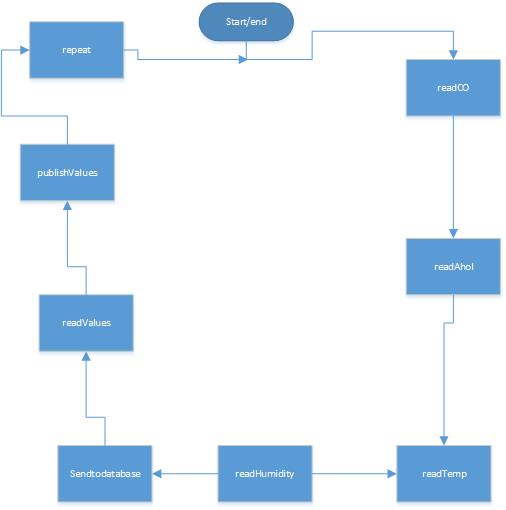
\includegraphics[scale=.3]{img/Fchatarduinomynd}
\end{figure}

\begin{figure}[h]
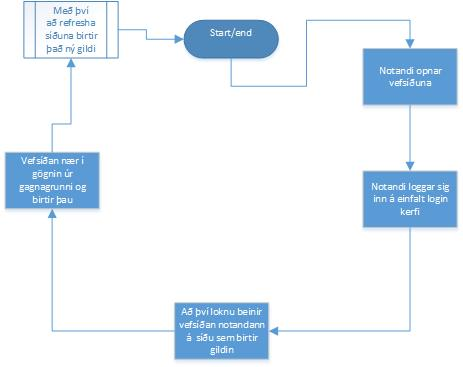
\includegraphics[scale=.3]{img/Fchatphpwebmynd}
\end{figure}

